\chapter{Analysis and comments}
\indent\indent
	In this project, a simple CNN model is implemented to recognize music notes. \\
	This CNN model is developed by \textbf{Python3} and \textbf{Keras}.
	
%%
\section{Network structure}
\indent\indent
	Network structure:
	\begin{enumerate}
		\item \textbf{32} convolutional layers with $4 * 4$ kernel size.
		\item A \textbf{RELU} activation function.
		\item \textbf{1} max pooling layer with $2 * 2$ kernel size.
		\item Dropout with \textbf{25\%} probability to prevent from over-fitting.
		\item A \textbf{256}-dimensions fully connected (FC) layer.
		\item A \textbf{RELU} activation function.
		\item Dropout with \textbf{50\%} probability.
		\item A \textbf{9}-dimensions fully connected (FC) layer to classify.
		\item A \textbf{Softmax} layer.
	\end{enumerate}

	\begin{figure}[H]
		\centering
		\label{anal_1}
		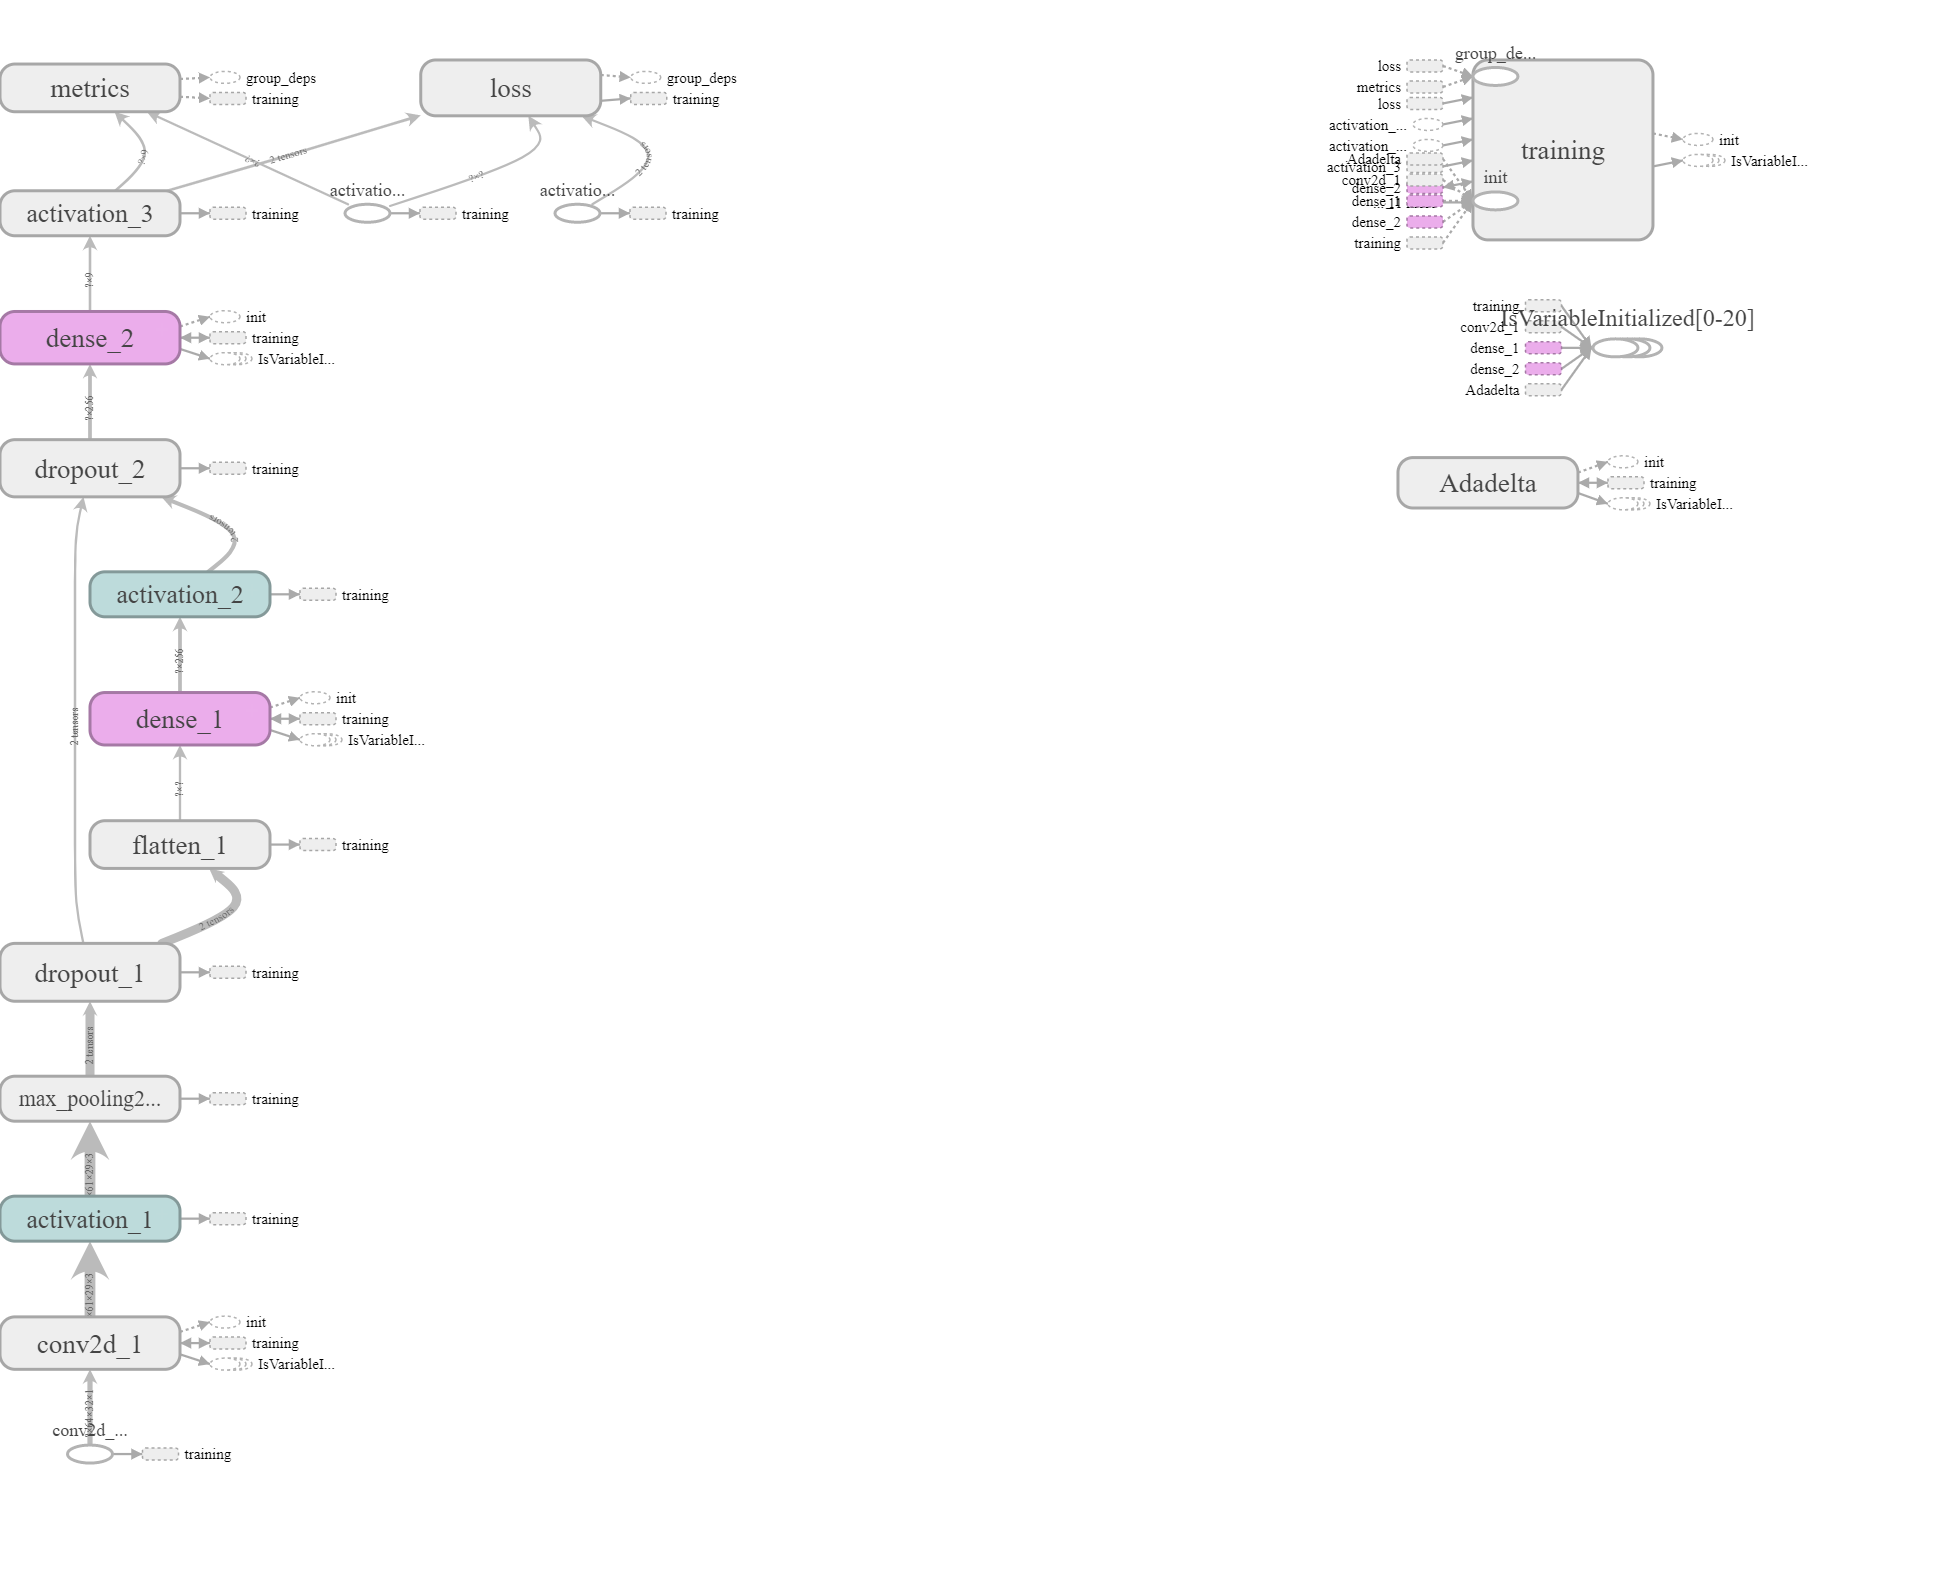
\includegraphics[scale=0.25]{img/sample_tensorboard.png}
		\caption{Tensorboard.}
	\end{figure}

%%
\section{Analysis}
\indent\indent
	In the figure \ref{anal_2}, the accuracy rate can be \textbf{98\%} in \textbf{8} epochs, and it shows the network structure works well for the testing data set.

	\begin{figure}[H]
		\centering
		\label{anal_2}
		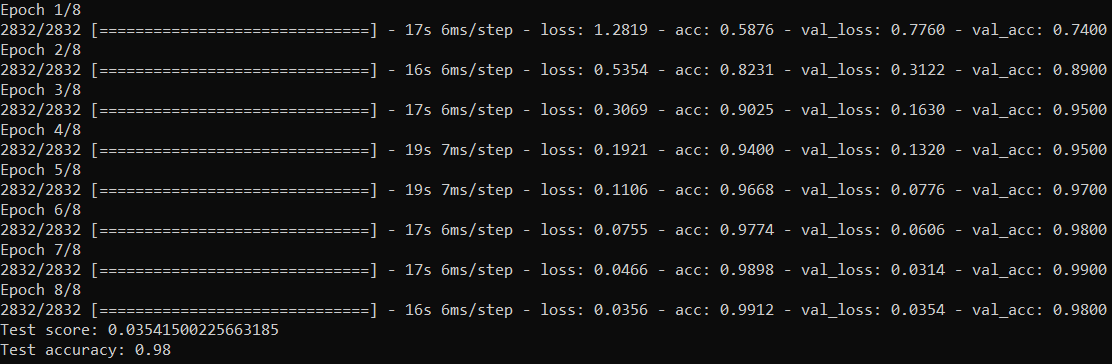
\includegraphics[scale=0.5]{img/sample_train_1.PNG}
		\caption{Accuracy rate.}
	\end{figure}
	

